

\section{Први домаћи задатак}
За руком писаних цифара 6, 8 и 9 која је доступна на сајту предмета испројектовати иновативни систем за препознавање цифара заснован на тестирању хипотеза. Резултате приказати у облику матрице конфузија. Извештај треба да садржи кратки опис испројектованог система, образложени избор обележја као и карактеристичне примере правилно и неправилно класификованих цифара
\subsection{Опис система}
На располагању налазило се 360 руком писаних цифара које су достављене у .bmp формату. Било је по 120 цифара 6, 8 и 9. Задатак је одрађен у програмском пакету \emph{Matlab vR2017b}.  Слике су обрађене у неколико фаза. 
	У првој фази одрађено је бинаризовање слике, тј. вредност свим пикселима је преведена да буде 255 или 0, с обзиром да је слика представљена као низ црних и белих пиксела различитих јачина. Бинаризација је одрађена функцијом \ref{fun:binarize}.
	
	

\renewcommand{\lstlistingname}{Одсечак кода}%
	
\begin{lstlisting}[caption={Бинаризација слике},label={fun:binarize}]
function [binImage] = binarizeImage(image, ratio)
    val = 255 - double(image);
    val(val < ratio * max(max(val))) = 0;
    val(val >= ratio * max(max(val))) = 255;
    binImage = uint8(255 - val);
end

\end{lstlisting}

\noindent Функција прима \emph{image} и \emph{ratio} који представљају дату слику, односно праг бељења-колика црнина се прихвата као белина.  
\\ \indent Друга фаза омогућава одсецање неискоришћеног простора, односно белина. Поред белина занемарене су све мрље унутар белина. Кад се каже мрља мисли се тачка величине бар 5 пиксела (в. сл. \ref{pic:dot6}, \ref{pic:dot8}, \ref{pic:dot9} као пример). 
\begin{figure}[htb!]\caption{Тачке}
\begin{subfigure}{.3\textwidth}
\centering
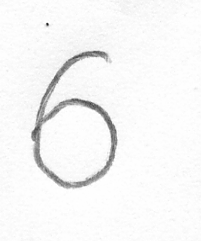
\includegraphics[width=.4\linewidth]{pictures/1/Dot6}
\caption{Тачка у 6}\label{pic:dot6}
\end{subfigure}
\begin{subfigure}{.3\textwidth}
\centering
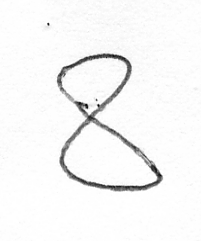
\includegraphics[width=.4\linewidth]{pictures/1/Dot8}
\caption{Тачка у 8}\label{pic:dot8}
\end{subfigure}
\begin{subfigure}{.3\textwidth}
\centering
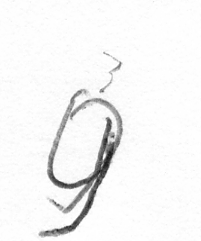
\includegraphics[width=.4\linewidth]{pictures/1/Dot9}
\caption{Тачка у 9}\label{pic:dot9}
\end{subfigure}
\end{figure}

Код за уклањање белина и тачки је одрађен функцијом \ref{fun:cropImage}.

\begin{lstlisting}[caption={Одсецање слике},label={fun:cropImage}]
function [X] = cropImage(image)
    ratio = 0.20;
    X = binarizeImage(image, ratio);
    
    [numRow, numCol] = size(X);
    begin = 1;
    while (begin < numRow) && (sum(X(begin, 1 : numCol)) / numCol > 250 ||...
            sum(X(begin + 1, 1 : numCol)) / numCol > 250 ||...
            sum(X(begin + 2, 1 : numCol)) / numCol > 250 ||...
            sum(X(begin + 3, 1 : numCol)) / numCol > 250 ||...
            sum(X(begin + 4, 1 : numCol)) / numCol > 250 ||...
            sum(X(begin + 5, 1 : numCol)) / numCol > 250)
        begin = begin + 1;
    end

    endV = numRow;
    while(endV > begin)&&...
            (sum(X(endV, 1 : numCol)) / numCol > 250 ||...
            sum(X(endV - 1, 1 : numCol)) / numCol > 250 ||...
            sum(X(endV - 2, 1 : numCol)) / numCol > 250 ||...
            sum(X(endV - 3, 1 : numCol)) / numCol > 250 ||...
            sum(X(endV - 4, 1 : numCol)) / numCol > 250 ||...
            sum(X(endV - 5, 1 : numCol)) / numCol > 250)
        endV = endV - 1;
    end

    left = 1;
    while (left < numCol)&&...
            (sum(X(1 : numRow, left)) / numRow > 250 ||...
            sum(X(1 : numRow, left + 1)) / numRow > 250 ||...
            sum(X(1 : numRow, left + 2)) / numRow > 250 ||...
            sum(X(1 : numRow, left + 3)) / numRow > 250 ||...
            sum(X(1 : numRow, left + 4)) / numRow > 250 ||...
            sum(X(1 : numRow, left + 5)) / numRow > 250)
        left = left + 1;
    end

    right = numCol;
    while (right>1)&&...
            (sum(X(1 : numRow,right)) / numRow > 250 ||...
            sum(X(1 : numRow, right - 1)) / numRow > 250 ||...
            sum(X(1 : numRow, right - 2)) / numRow > 250 ||...
            sum(X(1 : numRow, right - 3)) / numRow > 250 ||...
            sum(X(1 : numRow, right - 4)) / numRow > 250 ||...
            sum(X(1 : numRow, right - 5)) / numRow > 250)
        right = right - 1;
    end

    X = X(begin : endV, left : right);
end

\end{lstlisting}

Овде је коришћен $ratio= 0, 2$  јер даје најбољу тачност за одговарајући скуп података. Међутим и поред свега дође до лошег одсецања (в. сл. \ref{pic:badCrop6}, \ref{pic:badCrop8}).
\begin{figure}[htb!]
\caption{Лоше одсецање}
\begin{subfigure}{.5\textwidth}
\centering

\includegraphics[width=.5\linewidth]{pictures/1/BadCrop6}
\caption{Лоше одсецање 6}\label{pic:badCrop6}
\end{subfigure}
\begin{subfigure}{.5\textwidth}
\centering

\includegraphics[width=.3\linewidth]{pictures/1/BadCrop8}
\caption{Лоше одсецање 8}\label{pic:badCrop8}
\end{subfigure}
\end{figure}

У осталим исправним случајевима добију се бројеви као на сл.  \ref{pic:goodCrop6}, \ref{pic:goodCrop8}, \ref{pic:goodCrop9}.
\begin{figure}[htb!]\caption{Добро одсечене}
\begin{subfigure}{.3\textwidth}
\centering

\includegraphics[width=.4\linewidth]{pictures/1/GoodCrop6}
\caption{Добро одсечена цифра 6}\label{pic:goodCrop6}
\end{subfigure}
\begin{subfigure}{.26\textwidth}
\centering

\includegraphics[width=.4\linewidth]{pictures/1/GoodCrop8}
\caption{Добро одсечена цифра 8}\label{pic:goodCrop8}
\end{subfigure}
\begin{subfigure}{.3\textwidth}
\centering

\includegraphics[width=.48\linewidth]{pictures/1/GoodCrop9}
\caption{Добро одсечена цифра 9}\label{pic:goodCrop9}
\end{subfigure}
\end{figure}

Крајња, трећа фаза рачуна "центар масе" цифара добијених из друге фазе и формира функцију густине расподеле вероватноће за сваку од центара масе цифара 6, 8, 9. Центар маса се рачуна функцијом \ref{fun:calculateCenter}. Функција помера координатни почетак слике тако да буде у центру слике и онда сабира све вредности пиксела померене са одговарајућим вектором положаја. На крају се добијена вредност подели са бројем пискела на слици и то је центар масе дате слике.

\begin{lstlisting}[caption={Центар масе},label={fun:calculateCenter}]
function [center] = calculateCenter(X)
    [numRow, numCol] = size(X);
    centerX = 0;
    centerY = 0;
    for row = 1 : numRow
        for col = 1 : numCol
           val = floor(double(X(row, col)));
           centerX = centerX + val * (row - floor(numRow / 2));
           centerY = centerY + val * (col - floor(numCol / 2));
        end
    end
    center = [centerX; centerY] / (numRow * numCol);
end
\end{lstlisting}

Oбрада цифара за све 3 фазе одрађена је кодом \ref{piece:train}. Овде се може приметити да је узето 300 од 360 слика за тренирање, а 60 за проверу, што је $83\%-17\% $ однос у подели скупа на обучавајући и тренирајући скуп. 

\begin{lstlisting}[caption={Обрада цифара},label={piece:train}]
N = 100;
for i = 1 : N
    name = ['BazaCifara6/baza6' num2str(i, '%03d')];
    X = imread(name, 'bmp');    
    nameCropped = ['BazaCifaraCropped6/baza6' num2str(i, '%03d') '.bmp'];
    croppedImage = cropImage(X);
    imwrite(croppedImage, nameCropped, 'bmp');
    features6(:, i) = calculateCenter(croppedImage);
    
    name = ['BazaCifara8/baza8' num2str(i, '%03d')];
    X = imread(name, 'bmp');  
    nameCropped = ['BazaCifaraCropped8/baza8' num2str(i, '%03d') '.bmp'];
    croppedImage = cropImage(X);
    imwrite(croppedImage, nameCropped, 'bmp');
    features8(:, i) = calculateCenter(croppedImage);
    
    name = ['BazaCifara9/baza9' num2str(i, '%03d')];
    X = imread(name, 'bmp');  
    nameCropped = ['BazaCifaraCropped9/baza9' num2str(i, '%03d') '.bmp'];
    croppedImage = cropImage(X);
    imwrite(croppedImage, nameCropped, 'bmp');
    features9(:, i) = calculateCenter(croppedImage);
end

figure;
hold on
plot(features6(1, :), features6(2, :), 'sb');
plot(features8(1, :), features8(2, :), 'hg');
plot(features9(1, :), features9(2, :), 'ro');
legend('Sest', 'Osam', 'Devet');
title('Skup za obucavanje');
\end{lstlisting}

Приказ расподеле скупа тренирајућих цифара je приказано на слици \ref{fig:Train}.

\begin{figure}[htb!]

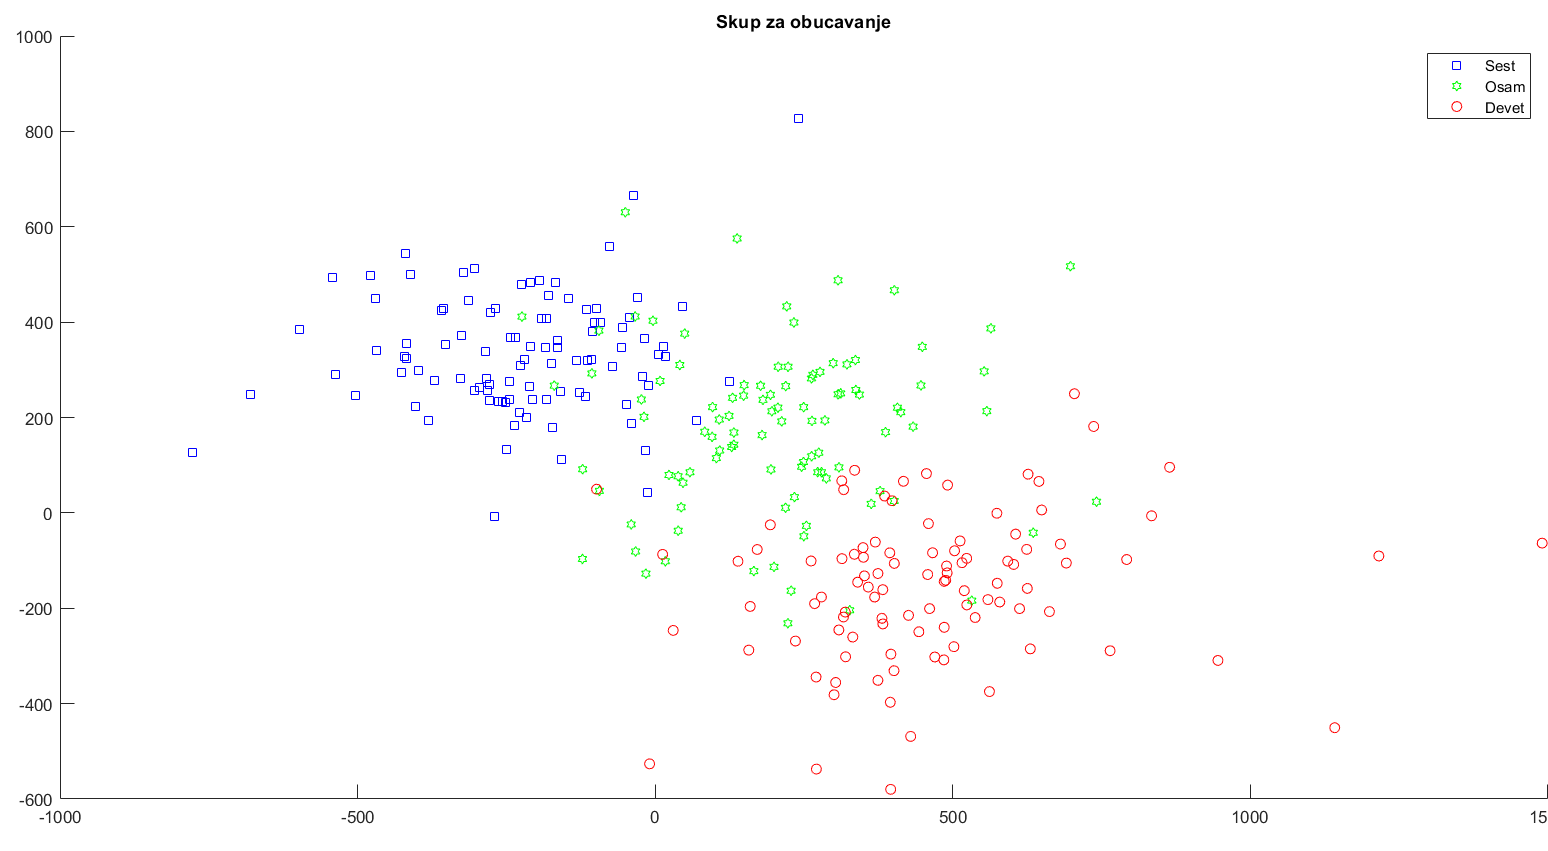
\includegraphics[scale=.42]{pictures/1/TrainSet}
\caption{Oбучавајући скуп}\label{fig:Train}
\end{figure}



Функција густине вероватноће за сваку цифру се рачуна тако што се израчунају математичка очекивања и варијансе за сваки од 3 скупа цифара (в. одсечак \ref{fun:calcExpVar}).

\begin{lstlisting}[caption={Варијансе и математичка очекивања},label={fun:calcExpVar}]
M1 = mean(features6')'; 
S1 = cov(features6');
M2 = mean(features8')'; 
S2 = cov(features8');
M3 = mean(features9')'; 
S3 = cov(features9');
\end{lstlisting}

И потом се израчунају 3 функције густине вероватноће за сваку цифру при чему се густина рачуна користећи функцију \ref{fun:gaus}, при чему се проследе одговарајућа математичка очекивања и коваријациона матрица.
\begin{lstlisting}[caption={Гаусова расподела},label={fun:gaus}]
function [Y] = gausianMultivariate(X, Mx, Sx)
n = size(Sx, 1);
Y = (1 / ((2 * pi) ^(n / 2)  * sqrt(det(Sx)))) * exp((X - Mx)' * inv(Sx) * (X - Mx) / -2);
end
\end{lstlisting}

У зависности која функција густине вероватноће је већа, тој класи припада цифра која се препознаје. Код за одлучивање којој класи припада је дат одсечком \ref{fun:test}.
\begin{lstlisting}[caption={Одлучивање припадности класи},label={fun:test}]
for k = 1:3
    if k == 1
        T = featuresTest6;
    elseif k == 2
        T = featuresTest8;
    else
        T = featuresTest9;
    end
    
    for i = 1 : size(T, 2)
        f1 = gausianMultivariate(T(:, i), M1, S1);
        f2 = gausianMultivariate(T(:, i), M2, S2);
        f3 = gausianMultivariate(T(:, i), M3, S3);
        if (f1 > f2) && (f1 > f3)
            CM(1, k) = CM(1, k) + 1;
            if (k ~= 1)
                fprintf("Predicted: 1 Actual: %d %d\n", k, i + N);
            end
        elseif f2 > f1 && f2 > f3
            CM(2, k) = CM(2, k) + 1;
            if (k ~= 2)
                fprintf("Predicted: 2 Actual: %d %d\n", k, i + N);
            end
        elseif f3 > f2 && f3 > f1
            CM(3, k) = CM(3, k) + 1;
            if (k ~= 3)
                fprintf("Predicted: 3 Actual: %d %d\n", k, i + N);
            end
        end
    end
end

\end{lstlisting}
Добијена матрица конфузије је у табели \ref{tab:matConf}.Можемо да приметимо да је $88,33$ прецизност оваквог препознавања. Такође можемо да приметимо да се 8 најчешће погрешно класификује (4 пута, а 6 и 9 збирно 3 пута су погрешно класификоване), што је за очекивати.
\begin{table}[h!] 
\centering
\caption{Матрица конфузије}\label{tab:matConf}
\vspace*{4mm}
\begin{tabular}{cc|c|c|c|l}
	\cline{3-5}
	& & \multicolumn{3}{ c| }{Стварно} \\ \cline{3-5}
	& & \textit{6} & \textit{8} & \textit{9}  \\ \cline{1-5}
	\multicolumn{1}{ |c  }{\multirow{3}{*}{Класификовано} } &
	\multicolumn{1}{ |c| }{\textit{6}}  & 18 & 3 & 0 &     \\ \cline{2-5}
	\multicolumn{1}{ |c  }{}                        &
	\multicolumn{1}{ |c| }{\textit{8}}  & 2 & 16 & 1 &     \\ \cline{2-5}
	\multicolumn{1}{ |c  }{}                        &
	\multicolumn{1}{ |c| }{\textit{9}}  & 0 & 1 & 19 &     \\ \cline{1-5}
\end{tabular}
\end{table}

\subsection{Избор обележја}
Избор "центра масе" као обележја за које ће се посматрати функција расподеле је разуман јер ако би се 6, 8, 9 и посматрали као објекти, могло би се приметити да је маса 6 пребачена у доњи део, док је за 8 у средњем, а за 9 у горњем, што се може приметити и на слици \ref{fig:Train} јер осмице су груписане око координатног центра, деветке су груписане у горњем делу (негативно за $y$ због тога што за слике је координатни систем обрнут код $y$) и шестице су груписане у доњем делу. Занимљиво је да ће груписање по $x$ оси за шестице и деветке бити симетрично у односу на координатни почетак, јер маса девет је углавном у "десном" крај, а шест у "левом" крају слике. 
\newpage
\subsection{Пример класификација}

\begin{figure}[htb!]\caption{Правилна класификација}
\begin{subfigure}{.3\textwidth}
\centering

\includegraphics[width=.4\linewidth]{pictures/1/GoodClass6}
\caption{Тачка у 6}\label{pic:goodClass6}
\end{subfigure}
\begin{subfigure}{.3\textwidth}
\centering

\includegraphics[width=.4\linewidth]{pictures/1/GoodClass8}
\caption{Тачка у 8}\label{pic:goodClass8}
\end{subfigure}
\begin{subfigure}{.3\textwidth}
\centering

\includegraphics[width=.4\linewidth]{pictures/1/GoodClass9}
\caption{Тачка у 9}\label{pic:goodClass9}
\end{subfigure}
\end{figure}


\begin{figure}[htb!]\caption{Неправилна класификација}
\begin{subfigure}{.3\textwidth}
\centering

\includegraphics[width=.4\linewidth]{pictures/1/BadClass6}
\caption{Класификована 8, а 6 је}\label{pic:goodClass6}
\end{subfigure}
\begin{subfigure}{.3\textwidth}
\centering

\includegraphics[width=.4\linewidth]{pictures/1/BadClass8}
\caption{Класификована 6, а 8 је}\label{pic:goodClass8}
\end{subfigure}
\begin{subfigure}{.3\textwidth}
\centering

\includegraphics[width=.4\linewidth]{pictures/1/BadClass9}
\caption{Класификована 8, а 9 је}\label{pic:goodClass9}
\end{subfigure}
\end{figure}












